% \documentclass[]{tMOP2e}
% 
% \citestyle{tMOP}
% \begin{document}
% 
% \doi{10.1080/0950034YYxxxxxxxx}
% \issn{1362-3044}
% \issnp{0950-0340} \jvol{00} \jnum{00} \jyear{2010} \jmonth{25 January}

%\markboth{A. Yamilov and B. Payne}{Classification of regimes of wave transport in quasi one-dimensional non-conservative random media}
 
\chapter{Classification of regimes of wave transport in quasi one-dimensional non-conservative random media}
\label{chap:regimes}
\label{paper:2_start}

% \author{
% A. Yamilov$^\ast$ \thanks{$^\ast$Corresponding author. Email: yamilov@mst.edu \vspace{6pt}} and 
% B. Payne\\\vspace{6pt}  {\em{Physics Department, Missouri University of Science and Technology, Rolla, MO USA}}}
% 
\begin{center}
Alexey Yamilov$^1$ and Ben Payne$^1$
\end{center}

\ \\
\begin{center}
\textit{$^1$Department of Physics, Missouri University of Science \& Technology,\\ Rolla, MO 65409}
%$^2$Department of Applied Physics, Yale University, New Haven, CT 06520}
\end{center}

\ \\
% \maketitle
% \begin{abstract}
% 
\addcontentsline{toc}{section}{ABSTRACT}
\begin{center}\textbf{ABSTRACT\footnote{Published in Journal of Modern Optics (2010)}}        \end{center}

Passive quasi-one-dimensional random media are known to exhibit one of the three regimes of transport -- ballistic, diffusive or localized --  depending on the system size. In contrast, in non-conservative systems the physical parameter space also includes the gain/absorption length scale. Here, by studying the relationships between the transport mean free path, the localization length, and the gain/absorption length, we enumerate fifteen regimes of wave propagation through quasi-one-dimensional random media with gain or absorption. The results are presented graphically in a form of a phase diagram. Of particular experimental importance, in absorbing random medium we identify three different regimes which bear signatures of the localized regime of the passive counterpart. We also review the literature and, when possible, assign experimental systems to a particular regime on the diagram. 
% \begin{keywords} 
% Wave propagation in random media; diffusion; Anderson localization; random laser
% \end{keywords}
% \end{abstract}

\section{INTRODUCTION}
\label{sec:introduction}

Discovery of Anderson localization (AL)~\cite{1958_Anderson} served as a catalyst for interest in wave propagation through random media for over fifty years~\cite{2009_Lagendijk_PT}. AL is a wave phenomenon~\cite{2007_Akkermans_book} that results in cessation of diffusion~\cite{2010_Wolfle}. First conceived in electronic systems, it originates from  repeated self-interference of de Broglie waves during their propagation in a random potential. Conservation of number of carriers, enforced because the electrons possess a charge, lies in the foundation of the concept of AL~\cite{1991_Altshuler}. 

Understanding the effect of absorption~\cite{1984_John_prl}, ubiquitous in optical systems, turned out to be essential for proper physical description and interpretation of experimental studies of localization of {\it light}~\cite{1989_Genack,1997_wiersma_nature,1999_Maret,2000_chabanov_nature,2007_Maret,2007_Segev} and other classical waves such as ultrasound~\cite{2008_van_Tiggelen_Nature,2008_Weaver}. It also prompted~\cite{2000_chabanov_nature} the search for alternative criteria of localization in absorbing media. Furthermore, the effect opposite to the absorption, coherent amplification, leads to an altogether new wave phenomenon of random lasing with a host of potential applications~\cite{2005_Cao,2008_Wiersma}. The multitude of the observed phenomena in realistic disordered optical systems, which are inevitably absorbing or can even be made amplifying, suggests that AL phenomenon is intrinsically more complex in non-conservative random media. It motivates refinement of the very concept of AL and its criteria in such systems~\cite{2010_Payne_loc_criterion}.

In this work, with the goal of establishing a criterion of Anderson localization in non-conservative quasi-one-dimensional (quasi-1D) random media, such as disordered waveguides, we map out the two-dimensional parameter space of the problem that consists of the system size and gain or absorption length. In quasi-1D geometry the transition to AL lacks sharp features (mobility edges) observed in even more complex three-dimensional systems. Thus,  Section \ref{sec:q1d_localization} is devoted to a discussion of Anderson localization in quasi-1D random media. In Section \ref{sec:parameters} we review and formally define the parameters that characterize quasi-1D non-conservative systems. In Section \ref{sec:phases}, by studying the relationships between these parameters we identify fifteen different regimes of wave transport in the parameter space. Furthermore, we review the available publications on the subject and, when published data is sufficient, assign them to a particular region on our phase-diagram. We conclude with a discussion of the results obtained in Section \ref{sec:discussion_regimes}.

\section{LOCALIZATION IN QUASI-1D NON- CONSERVATIVE RANDOM MEDIA}
\label{sec:q1d_localization}

\subsection{Localization in Finite Passive Random Media}

Anderson localization can be defined in a strict mathematical sense in random media with infinite dimensions~\cite{2010_Spencer}. In experimentally relevant situations, one usually deals with finite systems that are characterized by non-zero wave flux at the boundaries. Thus, a study of localization in finite systems is an analysis of transport through random media. 

The dimensionless conductance averaged over an ensemble of macroscopically equivalent, but microscopically different disorder realizations, $g$, can be used as a criterion that defines the onset of localization~\cite{1977_Thouless}. According to scaling theory of localization~\cite{1979_Anderson}, $g$  uniquely determines  evolution of its entire distribution with an increase of the system size, formally described by the scaling function~\cite{2010_Kramer}. Thus, the scaling theory provides an important link between finite and the infinite systems.

\subsection{Localization in Finite Random Media With Gain or Absorption}

Transmittance is the electromagnetic counterpart of conductance~\cite{1988_Stone}. This analogy with mesoscopic electronic transport makes it tempting to adopt the localization criteria (LC) based on $g$ in optical systems. However, the LC developed for passive systems are not necessarily applicable for non-conservative random media, where the extrapolation to infinite size becomes problematic~\cite{1999_van_Tiggelen}. The scaling function is no longer a single parameter function~\cite{1994_Freilikher_absorption}. Indeed, in absorbing systems $g\ll 1$ may not be indicative of the presence of localization~\cite{1998_Brouwer,2000_chabanov_nature}, and $g\gg 1$ in an amplifying random medium may not necessarily preclude occurrence of certain effects characteristic of localized systems~\cite{2004_Yamilov_intensity,2006_Yamilov_conductance}. Therefore, studies of localization in non-conservative systems concentrated on detecting the signatures of AL such as enhanced fluctuations~\cite{1994_Kumar,1995_Zhang,1996_Paasschens_gain,1997_Freilikher_gain,1998_Maret_PRL,2000_chabanov_nature,2006_Yamilov_conductance}, rounding of the coherent back scattering cone~\cite{1997_Wiersma_cbs,1999_Kaiser_cbs,2009_Maret}, anomalous diffusion~\cite{1989_Genack,1997_wiersma_nature,2006_Maret,2007_Segev,2008_van_Tiggelen_Nature,2009_Genack_PRB} and others.

In the case of absorption, a quantitative criterion, based on the magnitude of {\it fluctuation} of transmission normalized by its average, was put forward~\cite{2000_chabanov_nature}. Although it described the experiment well, the assumed critical value of fluctuations is somewhat subjective. In view of the fact that single parameter scaling is no longer applicable in presence of absorption~\cite{1994_Freilikher_absorption}, it remains an open question whether the same criterion would be suitable for systems with different values of absorption. 

In random media with gain, the situation is further complicated because within the statistical ensemble there always exists a non-zero probability of encountering a special realization of disorder where the given value of the gain parameter exceeds threshold for random lasing. Without saturation effects, such a realization will have an infinite contribution to the statistical average. Inclusion of saturation introduces dependence on system- and material-specific parameters which are not associated with wave-transport properties of the random medium. To regularize the statistical ensemble, conditional statistical averaging was introduced by excluding the diverging contributions~\cite{2005_Yamilov_correlations}. Such an approach turned out to be fruitful in studies of enhanced fluctuations and  correlation in mesoscopic transport of the electromagnetic waves through random media with optical amplification~\cite{2004_Yamilov_intensity,2006_Yamilov_conductance,2005_Yamilov_correlations}. It was found that the correlation linewidth $\delta\omega$~\cite{2000_Sebbah} obtained in such an ensemble can be used to define the Thouless parameter $\delta=\delta\omega/\Delta\omega$ in random media with gain. Here $\Delta\omega$ is the average mode spacing which is equal to the reciprocal of the density of states in the system.  Reduction of $\delta$ correlates well~\cite{2005_Yamilov_correlations} with the enhancement of mesoscopic fluctuations -- another signature of AL. These investigations motivated us to explore an intriguing possibility of localization by gain -- enhancement of the mesoscopic phenomena with an increase of the amplification strength. Because the dimensionless conductance and Thouless parameter exhibit opposite trends with an increase of gain, the relationship $g=\delta$ is no longer valid in non-conservative media. This observation exemplifies added complexity in description of wave propagation in open random media with gain (or absorption), even when such effects as gain saturation or spontaneous emission noise (see e.g. Refs.~\cite{1999_Patra_noise,2009_Skipetrov_noise}) are not accounted for.

\subsection{Disordered Waveguide (Wire) Geometry}

Because of quantization of the transverse component of momentum, the transport properties in quasi-1D (waveguide)  geometry can be conveniently described in terms of a transfer matrix~\cite{1997_Beenakker}. Assuming that this transfer matrix has random entries with only flux and symmetry conservation turned out to be a fruitful approach~\cite{2004_Mello_Kumar_book} which yielded some exact analytical results~\cite{1994_Beenakker_exact,2000_Mirlin}.

In passive quasi-1D systems the transition from ballistic to diffusive and then to localized regimes occurs as a function of the system size $L$ only (and not the strength of disorder as in three-dimensions, 3D), even if the system is weakly scattering $k\ell\gg 1$. The diffusion regime is only a transitive regime which, unlike in 3D systems, does not persists in the limit $L\rightarrow\infty$. Therefore, quasi-1D systems 
\cite{1995_Kogan,1996_Paasschens_gain,1998_Brouwer,1998_Birman_waveguide,1998_Maret_PRL,1999_Muttalib,
2000_chabanov_nature,2002_Saenz_g,2005_Markos,2005_Genack_review,2006_Yamilov_conductance,2007_Botten_waveguide,
2007_Froufe-Perez_PRE,2007_deMatos_random_fiber_laser} do not exhibit critical behavior at the size-driven transition from diffusive to localized transport. However, because we set out to consider the non-conservative systems for which $L\rightarrow\infty$ may not be easily defined, quasi-1D geometry is sufficiently complex to capture both diffusive and localized behavior in systems of {\it finite size}. As shown below, it is expected to exhibit very complex parameter space, c.f. Fig.~\ref{fig:phase_space}. Furthermore, due to the availability of the ever more powerful computational resources, it has recently become possible to perform systematic numerical investigations of the entire parameter space of the quasi-1D non-conservative random media. 

Although an interplay between the effects of amplification and localization has been subject of continuous research effort (see e.g. Refs.~\cite{1994_Kumar,1995_Zhang,1995_zyuzin_fluctuations,1996_Paasschens_gain,1997_Freilikher_gain,1997_Wiersma_cbs,
2000_Cao_localization,2001_Soukoulis_modeDist,2001_Sebbah_FDTD,2004_Yamilov_intensity,2005_Genack_Milner,
2005_Apalkov_corr,2005_Yamilov_correlations,2006_Heinrichs,2006_Yamilov_conductance,2008_Stone,2008_Conti_opals,
2009_Frank,2010_Payne_PRL}), a systematic study which would rationalize different theoretical and experimental observations has not yet been attempted. Below, we present such a systematic analysis of the parameter space for quasi-1D non-conservative random media.

%-----------------------------------------------
\section{DEFINITIONS OF PARAMETERS IN QUASI-1D NON- CONSERVATIVE RANDOM MEDIA}
\label{sec:parameters}
%-----------------------------------------------

% %%%%%%%%%%%%%%%%%%%%%%%%%%%%%%%%%%%%%%%%%%%%
% \begin{figure}
% \vskip -0.2cm
% \centerline{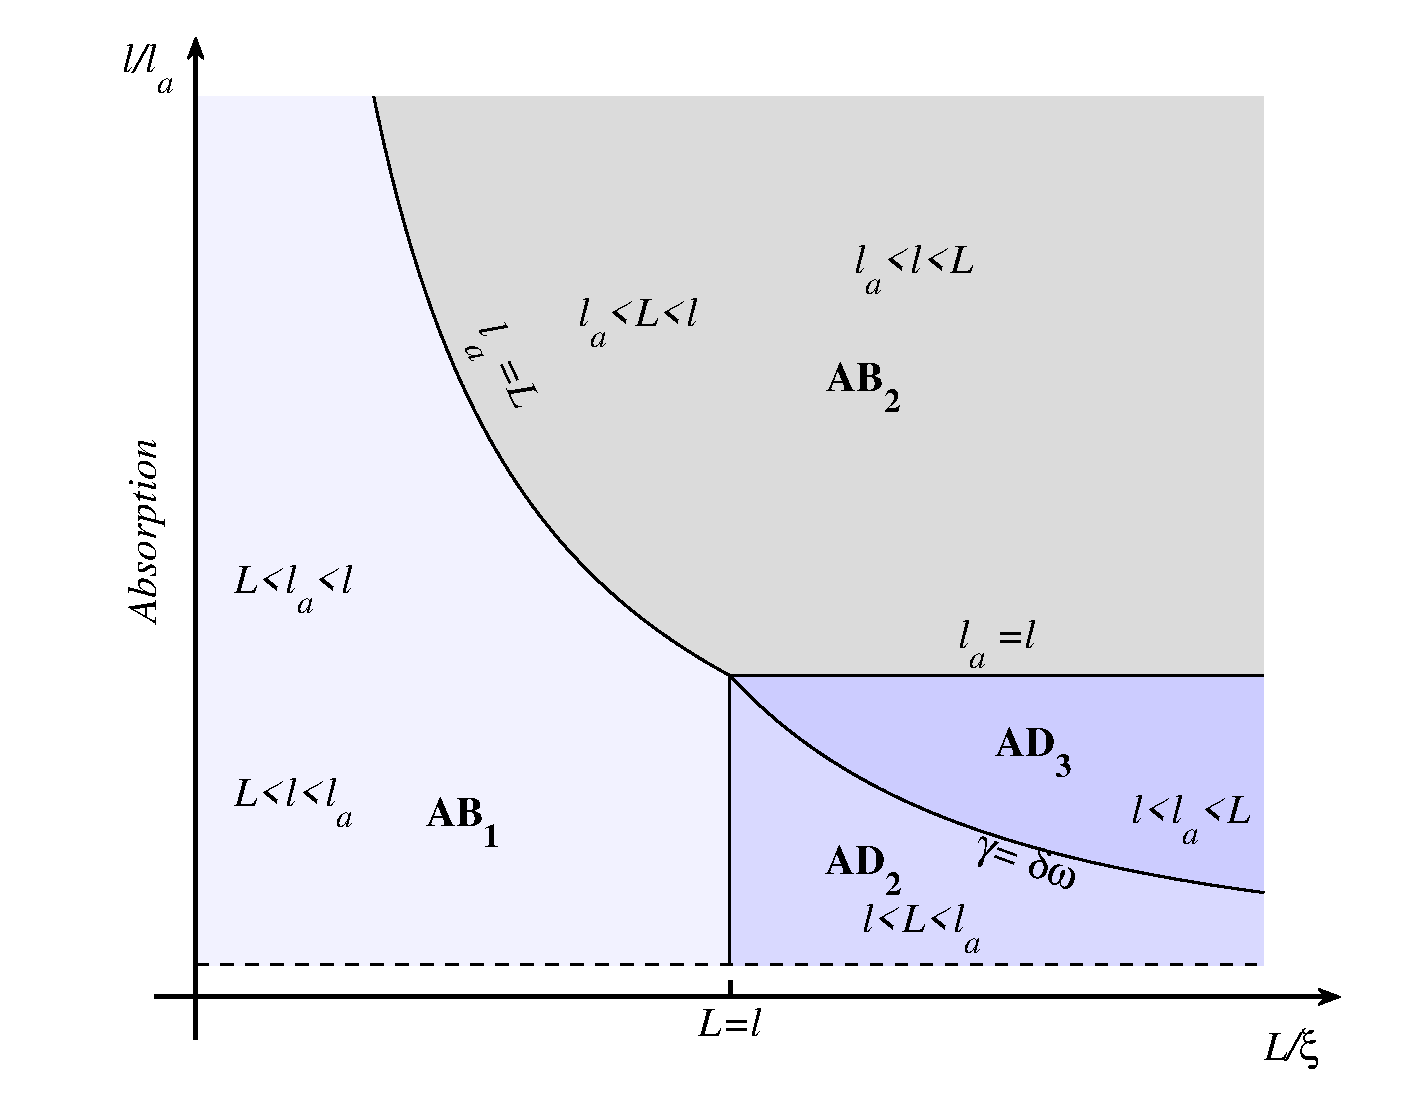
\includegraphics[width=4in]{chapters/Classification_of_regimes_of_wave_transport_in_non-conservative_random_media__J_Mod_Optics/pictures/fig1a_regimes_plot_upper}}
% \vskip -0.8cm
% \hskip -0.1cm
% \centerline{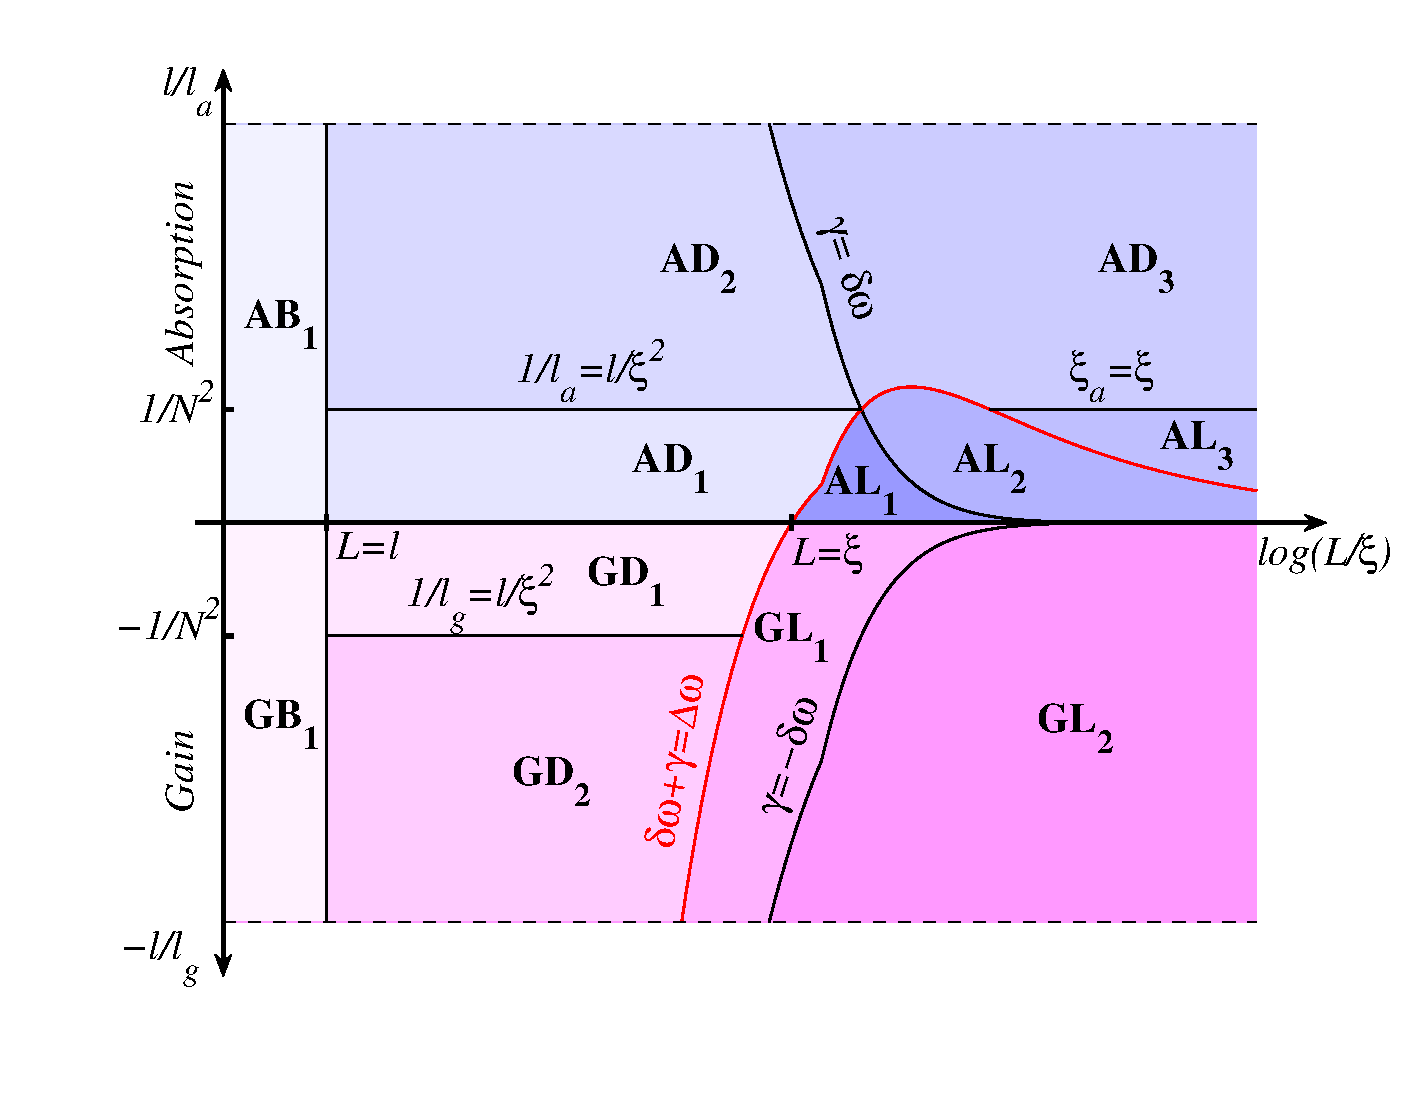
\includegraphics[width=4.15in]{chapters/Classification_of_regimes_of_wave_transport_in_non-conservative_random_media__J_Mod_Optics/pictures/fig1b_regimes_plot_main}}
% \vskip -0.6cm
% \centerline{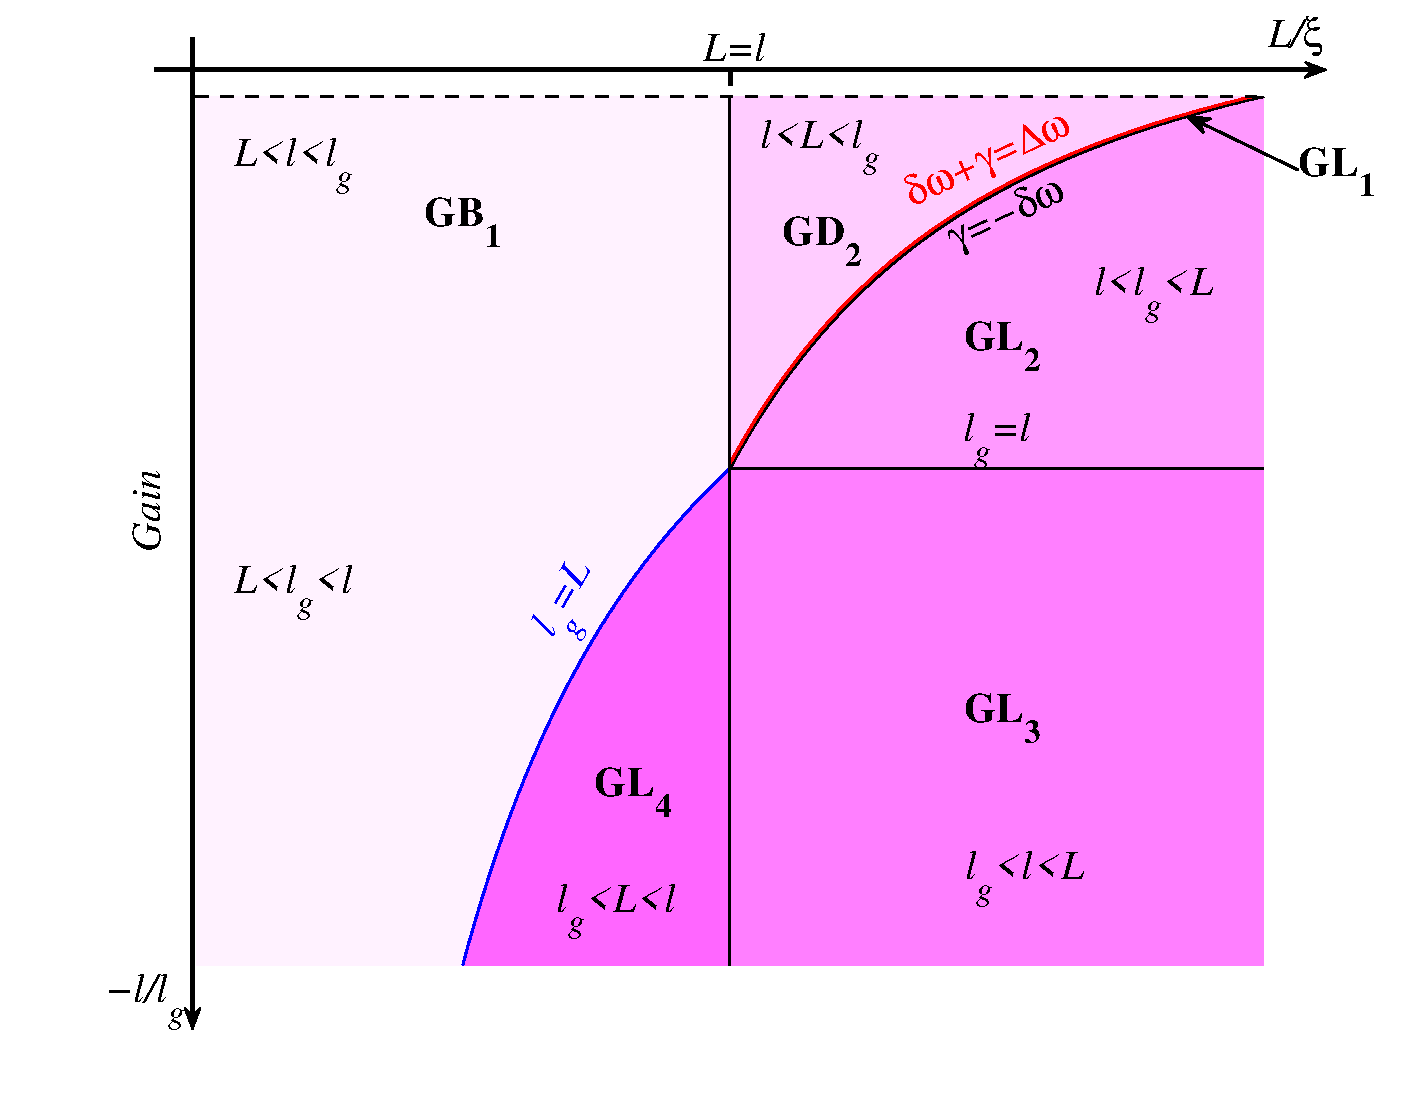
\includegraphics[width=4in]{chapters/Classification_of_regimes_of_wave_transport_in_non-conservative_random_media__J_Mod_Optics/pictures/fig1c_regimes_plot_lower}}
% \vskip -0.2cm
% \caption[Classification of regimes of wave transport in quasi-1D non-conservative random media.]{\label{fig:phase_space} Classification of regimes of wave transport in quasi-1D non-conservative random media. X and Y axes correspond to the system length $L$ and absorption/gain length $\ell_{a,g}$, see text for labeling convention. Due to large disparity in the characteristic length scales, the plot is separated into three panels which correspond to strong absorption $1/\ell_a\sim 1/\ell$ (upper panel), weak absorption and gain $1/\ell_{a,g}\sim \ell/\xi^2$ (middle panel), and strong gain $1/\ell_g\sim 1/\ell$ (lower panel) regimes. }
% \end{figure}
% %%%%%%%%%%%%%%%%%%%%%%%%%%%%%%%%%%%%%%%%%%%%%

%%%%%%%%%%%%%%%%%%%%%%%%%%%%%%%%%%%%%%%%%%%%
\begin{figure}
\vskip -0.2cm
\centerline{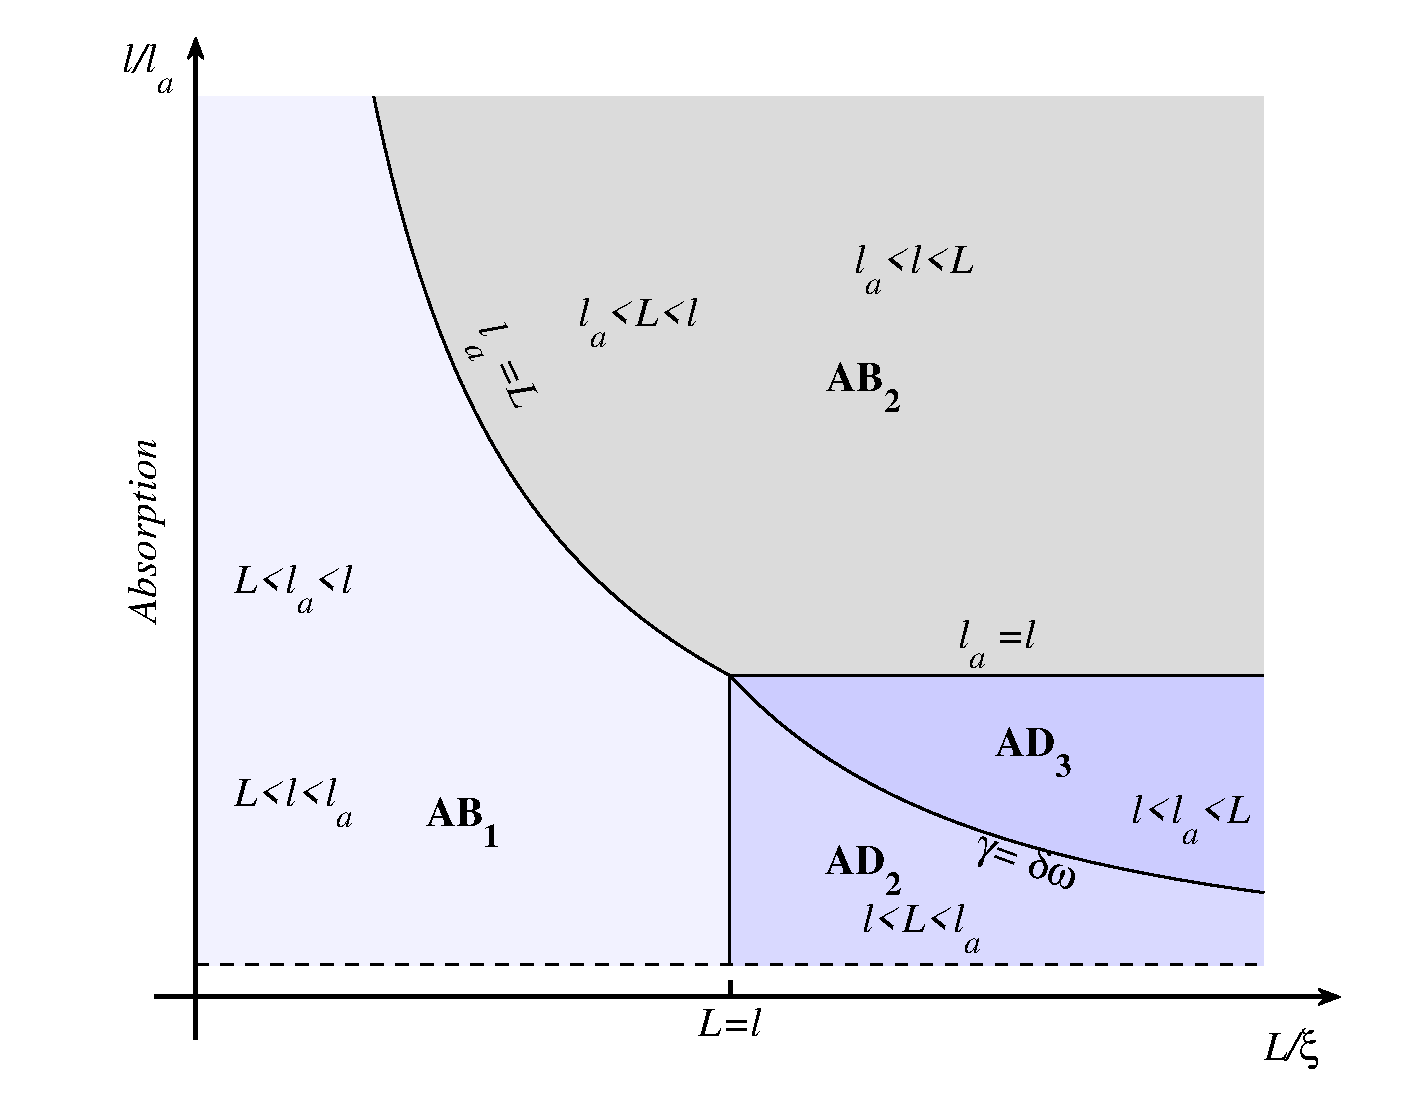
\includegraphics[width=4in]{chapters/Classification_of_regimes_of_wave_transport_in_non-conservative_random_media__J_Mod_Optics/pictures/fig1a_regimes_plot_upper}}
\vskip -0.2cm
\caption[Classification of regimes of wave transport in quasi-1D non-conservative random media; upper panel.]{Classification of regimes of wave transport in quasi-1D non-conservative random media; upper panel.}
\end{figure}

\begin{figure}
\hskip -0.1cm
\centerline{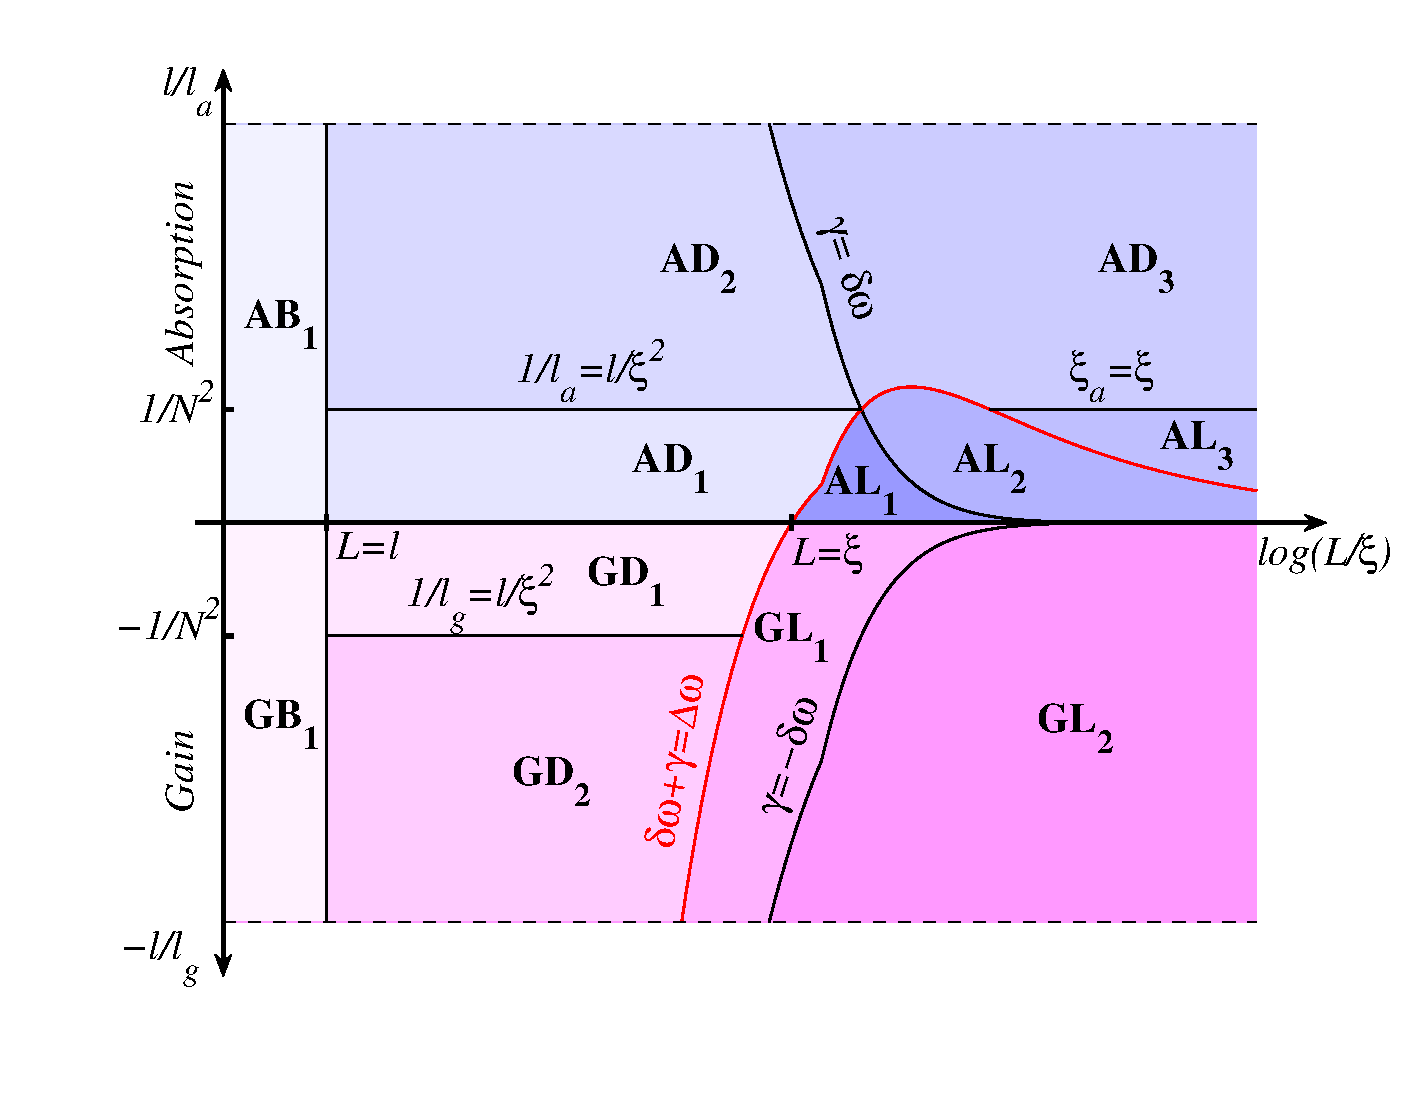
\includegraphics[width=4.15in]{chapters/Classification_of_regimes_of_wave_transport_in_non-conservative_random_media__J_Mod_Optics/pictures/fig1b_regimes_plot_main}}
\caption[Classification of regimes of wave transport in quasi-1D non-conservative random media; middle panel.]{Classification of regimes of wave transport in quasi-1D non-conservative random media; middle panel.}
\end{figure}

\begin{figure}
\vskip -0.6cm
\centerline{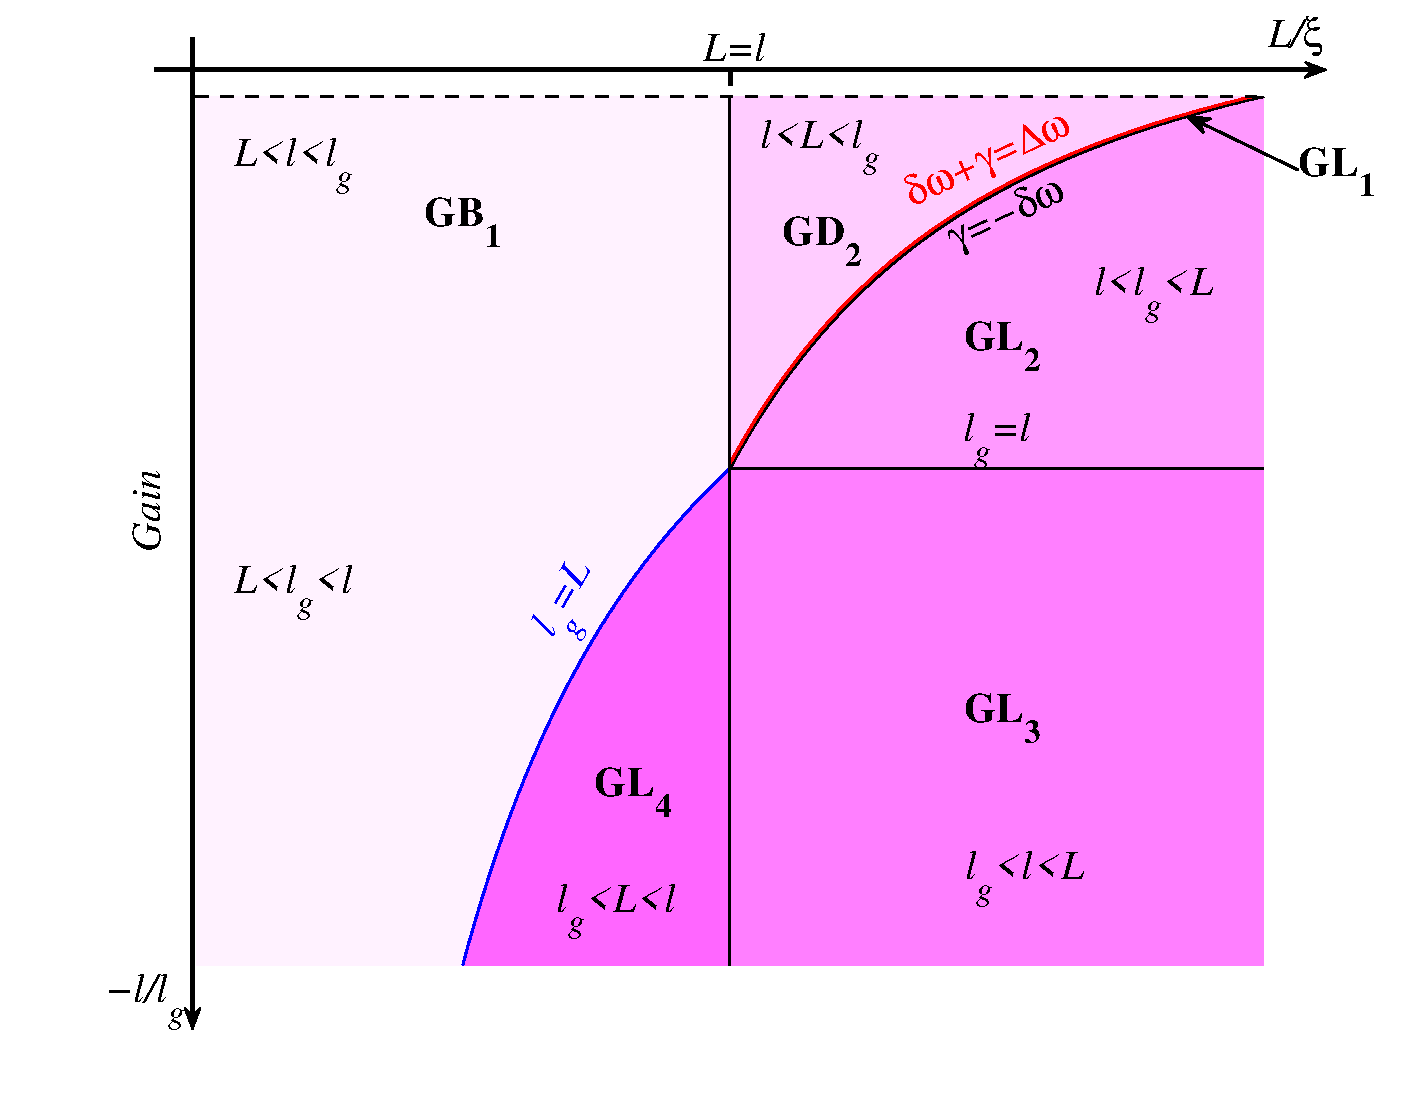
\includegraphics[width=4in]{chapters/Classification_of_regimes_of_wave_transport_in_non-conservative_random_media__J_Mod_Optics/pictures/fig1c_regimes_plot_lower}}
\vskip -0.2cm
\caption[Classification of regimes of wave transport in quasi-1D non-conservative random media; lower panel.]{\label{fig:phase_space} Classification of regimes of wave transport in quasi-1D non-conservative random media; lower panel. X and Y axes correspond to the system length $L$ and absorption/gain length $\ell_{a,g}$, see text for labeling convention. Due to large disparity in the characteristic length scales, the plot is separated into three panels which correspond to strong absorption $1/\ell_a\sim 1/\ell$ (upper panel), weak absorption and gain $1/\ell_{a,g}\sim \ell/\xi^2$ (middle panel), and strong gain $1/\ell_g\sim 1/\ell$ (lower panel) regimes. }
\end{figure}
%%%%%%%%%%%%%%%%%%%%%%%%%%%%%%%%%%%%%%%%%%%%%

In passive volume-disordered waveguides, the transition from ballistic to diffusive and then to the localized regime occurs when the length of the system is increased above $\ell$ and $\xi=N\times\ell$ respectively. Here $\ell$ is the transport mean free path, $N$ is the number of waveguide channels, and $\xi$ is the localization length~\cite{1997_Beenakker}. In waveguides filled with a non-conservative random medium, the parameter space becomes two-dimensional: beside the system size $L$, it also includes the gain or absorption length scale $\ell_{g,a}$. Fig.~\ref{fig:phase_space} shows this two-parameter phase space.

The boundaries between different regions in Fig.~\ref{fig:phase_space} are based on relationships between a subset of parameters which can be expressed in terms of length or time scales. The length parameters include $L$, $\ell$, $\xi$, and (ballistic) absorption/gain lengths $\ell_a/\ell_g$. The other set of boundaries are more physically transparent when expressed in the spectral domain in terms of the following parameters: the average mode spacing $\Delta\omega\propto (NL)^{-1}$; the passive average mode linewidth $\delta\omega$ ($\propto DL^{-2}$ in diffusive regime $\ell<L<\xi$); and gain or absorption rate $\gamma_{g,a}=\mp c/\ell_{g,a}\equiv\mp\tau_{g,a}^{-1}$ (negative in the case of gain). Here, $c$ is speed of light and $D$ is the diffusion constant. Based on these parameters the following relationships can be established:
\begin{quote}
$\bullet$ $L\sim\ell$ signifies the transition from ballistic to multiple-scattering regime. No other significant changes are expected in the region of moderate absorption/gain $\ell<\ell_{g,a}$ shown in the middle panel in Fig.~\ref{fig:phase_space};\\
$\bullet$ Generalized Thouless parameter $\delta\omega(\gamma)/\Delta\omega\simeq(\delta\omega+\gamma)/\Delta\omega$ describes~\cite{2005_Yamilov_correlations} the transition from spectrally overlapping quasi-modes to the resonance-dominated behavior. Here $\delta\omega\equiv\delta\omega(\gamma=0)$. In the case of passive system $\gamma=0$, the ratio reduces to $\delta=g$;\\
$\bullet$ $|\gamma|=\delta\omega$ curves signify the transition to the regime when the gain or absorption overcomes the radiative leakage of an average quasi-mode in the system;\\
$\bullet$ Long self-crossing Feynman paths give rise to weak localization correction. In quasi-1D, the probability of such paths becomes equal to unity at $L=\xi$, their length is given by $L^2/\ell=\xi^2/\ell$. Therefore, we estimate that the weak localization corrections become susceptible to gain or absorption when $\ell_{g,a}$ becomes comparable to this length scale;\\
$\bullet$ Condition $\ell=\ell_{g,a}$ marks the onset of the regimes of very strong absorption/gain shown in the upper/lower panel in Fig.~\ref{fig:phase_space}. Here, the ballistic regimes become limited by the condition $\ell_{g,a}=L$.\\
\end{quote}
\noindent The distinctions between different regions are only valid in the statistical sense because the sample-to-sample fluctuations are inherent in a random medium. When gain is present, the statistical ensemble is assumed to be conditional~\cite{2005_Yamilov_correlations}, which excludes the non-physical solutions~\cite{2002_Zhang_phys_solutions}. Furthermore, the considered (open) system is of a finite size and, therefore, the transitions between different ``phases'' are expected to be smooth. Hence, our diagrams should only be used as a guide to identify qualitatively different regimes of wave transport.

\section{``PHASES'' OF WAVE TRANSPORT THROUGH \\NON-CONSERVATIVE RANDOM MEDIA} 
\label{sec:phases}

The regions in Fig.~\ref{fig:phase_space} are labeled with two letters and a subscript. The first letter, $A/G$, stand for {\underline a}bsorption/{\underline g}ain and is common for all regions above/below the horizontal axis. The second letter in the labels, $B$, $D$ or $L$, is attributed to the regimes where some signatures of the {\underline b}allistic, {\underline d}iffusive, and {\underline l}ocalized transport are expected to occur. Based on the list of separatrices listed above, one can identify the following regions:
\begin{quote}
$\bullet$ $GB_1,AB_1$: Random systems with parameters in these regions are expected to behave similar to their passive counterparts. Note that in the regime of very strong gain or absorption, $\ell_{g,a}^{-1}>\ell^{-1}$, the ballistic region becomes bounded by $L<\ell_{g,a}$;\\
$\bullet$ $GD_1,AD_1$: With exception of anomalously localized states~\cite{1991_Altshuler,1995_Muzykantskii_ALS,2000_Mirlin,2000_Cao_localization,2002_Apalkov_ALS,2004_Burin_ALS}, the gain or absorption is not expected to be sufficient to appreciably modify the diffusive behavior in these regions; \\
$\bullet$ $GD_2$: Such systems were successfully treated with the ``negative absorption'' diffusive approach often invoked in discussion of random lasers~\cite{1968_Letokhov,1994_lawandy_nature,1996_John_RandLaser,1996_Wiersma_RandomLaser,1996_Genack_DiffRandomLaser,
1999_Cao_RandomLaserPRL,1999_Vardeny_PolymerRandomLaser,2001_vansoest_thesis,2004_Florescu}. Systems in this regime also are expected to exhibit the enhanced mesoscopic fluctuations and non-local correlations~\cite{2005_Yamilov_correlations,2004_Yamilov_intensity,2006_Yamilov_conductance};\\
$\bullet$ $GL_1$: Random media with such strong gain, $\delta\omega(\gamma)/\Delta\omega<1$, are expected to exhibit resonant features in spectrum with strong sample-to-sample fluctuations~\cite{1995_zyuzin_fluctuations,1997_Burkov_Zyuzin}. Retaining the contribution from only the physical solutions becomes essential~\cite{1999_Jiang,2002_Zhang_phys_solutions} for the systems with the parameters in this region;\\
$\bullet$ $GL_2$: The condition $\gamma_g=-\delta\omega(\gamma =0)$ signifies lasing of an average mode and, in diffusive systems, is equivalent to the onset random lasing as predicted by Letokhov~\cite{1968_Letokhov}; \\
$\bullet$ $AL_1,AL_2,AL_3$: These regimes represent the systems which would formally be localized if the absorption could be removed. Of these, $AL_1$ is the most favorable case because the systems in this regime have spectrum of separated resonances, $\delta\omega(\gamma)/\Delta\omega\simeq(\delta\omega(\gamma=0)+\gamma)/\Delta\omega<1$, with the radiative leakage being the dominant relaxation mechanism (possibly, experimental systems of~\cite{2000_chabanov_nature} belong to this parameter ``phase''). The latter is no longer true for $AL_2$ regime. $AL_3$ describes an intriguing type of a random medium with a continuous spectrum due to strong absorption which has washed out the individual resonances, but still exhibiting the weak localization corrections;\\
$\bullet$ $AD_2,AD_3$: Systems in these regimes of moderate and strong absorption are expected to exhibit suppressed localization effects~\cite{1998_Brouwer}. For strong absorption, even the diffusion propagation is suppressed on long scales. The majority of experimental systems are expected to fall in one of these two regions;\\
$\bullet$ $AB_2$: This regime is marked by the dominant effect of absorption when $\ell_a$ is the shortest of all length-scales. Because it also implies $\ell_a^{-1}>\ell^{-1}$, diffusion-like propagation does not sets in;\\
$\bullet$ $GL_3,GL_4$: In these regimes, similar to $GL_2$, it is more meaningful to ascribe $L$ notation to {\underline l}asing. In contrast to the very strong absorption counterpart $AB_2$, we separated $\ell_g^{-1}>\ell^{-1}$ region into $\ell_g<\ell<L$ ($GL_3$) and $\ell_g<L<\ell$ ($GL_4$). In the latter regime, one can justify neglecting scattering. Thus, $GL_4$ encompasses lasing phenomena in Fabry-Perot geometry. In contrast, in $GL_3$ the scattering can provide the dominant feedback as it has been very recently demonstrated experimentally~\cite{2006_Wu,2006_Wu_spie}.\\
\end{quote}
% Unlike the absorbing systems where one loc-abs, gain diff-loc\\

\section{DISCUSSION AND OUTLOOK}
\label{sec:discussion_regimes}

As it was discussed in the previous section, the parameter space in volume-disordered waveguides becomes two-dimensional when the medium is no longer assumed passive. Importantly, the coherent amplification/absorption non-trivially affects the interferences of multiply-scattered waves and, thus, can promote/suppress localization phenomena. This observation has motivated us to begin to systematically explore an intriguing possibility of localization by gain enhancement of the mesoscopic phenomena with an increase of the amplification strength~\cite{1995_zyuzin_fluctuations,1997_Burkov_Zyuzin,2004_Yamilov_intensity,2005_Yamilov_correlations,2006_Yamilov_conductance,2010_Payne_loc_criterion,2010_Payne_TE}. Furthermore, in the experimental studies of localization of light, the importance of the proper account of absorption has been widely appreciated~\cite{1991_Genack,1997_wiersma_nature,1999_Maret,2000_chabanov_nature,2006_Maret}. 

In finite {\it passive} random media, the prevalence of the localization effects can be assessed with a number of criteria: averaged dimensional conductance, its mesoscopic fluctuations relative to the mean value, Thouless parameter, renormalization of the diffusion coefficient, inverse participation ratio, spatial correlations and others. Single parameter scaling theory of localization may be used to establish the relationships between different criteria. These relationships will not necessarily hold in the non-conservative media. We believe that our analysis of the parameter space in Sec.~\ref{sec:phases} will be instrumental in generalizing the concept of AL and establishing a robust criterion for its observation in {\it non-conservative} random media~\cite{2010_Payne_loc_criterion,2010_Payne_TE}.

\section{ACKNOWLEDGMENTS}
This work was supported by National Science Foundation Grant No. DMR-0704981. 
%The numerical results that contributed to this work were obtained at the Tera-Grid, award no. DMR-090132.

% \bibliographystyle{tMOP}
% %\bibliography{C:/SVNr/research/latex_bibliography}
% \bibliography{20100712_regimes_plot.bbl}

%\end{document}
